\documentclass[tikz,border=2pt]{standalone}
\usepackage{amsmath}
\usepackage{pgfplots}
\pgfplotsset{compat=1.18}
\usetikzlibrary{arrows.meta}
\begin{document}
% Recycling: x = (1, 2) is repeated to the length of y. Against length 4: x - y = (0, 0, -2, -2),
% no message. Against length 5: the last copy is cut, x - y = (0, 0, -2, -2, -4) with a warning.
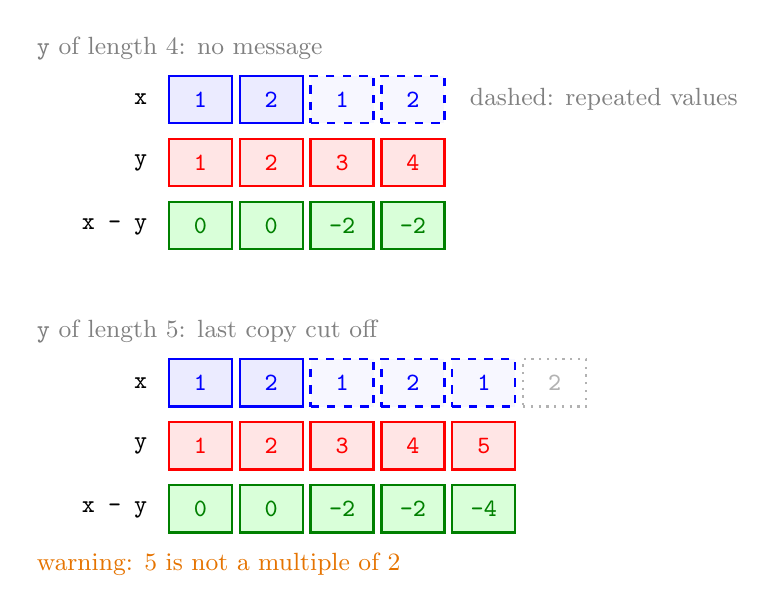
\begin{tikzpicture}[font=\small, >={Latex[length=2mm]},
  cell/.style={draw, thick, minimum width=8mm, minimum height=6mm, inner sep=0pt, font=\small\ttfamily}]
  % top panel
  \node[anchor=west, gray] at (-1.3,3.75) {\texttt{y} of length 4: no message};
  \foreach \v [count=\i] in {1,2,1,2} {
    \ifnum\i<3
      \node[cell, blue, fill=blue!8] at (0.9*\i,3.1) {\v};
    \else
      \node[cell, blue, dashed, fill=blue!3] at (0.9*\i,3.1) {\v};
    \fi
  }
  \foreach \v [count=\i] in {1,2,3,4} \node[cell, red, fill=red!10] at (0.9*\i,2.3) {\v};
  \foreach \v [count=\i] in {0,0,-2,-2} \node[cell, green!50!black, fill=green!15] at (0.9*\i,1.5) {\v};
  \node[anchor=east] at (0.35,3.1) {\texttt{x}};
  \node[anchor=east] at (0.35,2.3) {\texttt{y}};
  \node[anchor=east] at (0.35,1.5) {\texttt{x - y}};
  \node[gray, anchor=west] at (4.2,3.1) {dashed: repeated values};
  % bottom panel
  \begin{scope}[yshift=-3.6cm]
    \node[anchor=west, gray] at (-1.3,3.75) {\texttt{y} of length 5: last copy cut off};
    \foreach \v [count=\i] in {1,2,1,2,1} {
      \ifnum\i<3
        \node[cell, blue, fill=blue!8] at (0.9*\i,3.1) {\v};
      \else
        \node[cell, blue, dashed, fill=blue!3] at (0.9*\i,3.1) {\v};
      \fi
    }
    \node[cell, gray!60, dotted] at (5.4,3.1) {2};
    \foreach \v [count=\i] in {1,2,3,4,5} \node[cell, red, fill=red!10] at (0.9*\i,2.3) {\v};
    \foreach \v [count=\i] in {0,0,-2,-2,-4} \node[cell, green!50!black, fill=green!15] at (0.9*\i,1.5) {\v};
    \node[anchor=east] at (0.35,3.1) {\texttt{x}};
    \node[anchor=east] at (0.35,2.3) {\texttt{y}};
    \node[anchor=east] at (0.35,1.5) {\texttt{x - y}};
    \node[orange!90!black, anchor=west] at (-1.3,0.8) {warning: 5 is not a multiple of 2};
  \end{scope}
\end{tikzpicture}
\end{document}
